% Chapter X

\chapter{The ATLAS Detector} % Chapter title

\label{ch:atlas} % For referencing the chapter elsewhere, use \autoref{ch:name} 

The \acf{ATLAS} detector circumscribes the \ac{LHC}'s beam pipe, enclosing the collision point with a series of particle detecting layers, aimed at making as many measurements of the particles leaving the collision point as possible. Its goal is to get a precise measurement of all the stable or semi-stable particles flying from proton-proton collisions at its center, allowing analyzers to fully reconstruct the kinematics of the underlying processes.

The \ac{ATLAS} detector is the largest detector of its kind, measuring 44 m in length and 25 m in height, as seen in \autoref{fig:detector}. The size is mainly determined by the constraints of the \acf{MS}, discussed in \autoref{sec:MS}, which is the largest and outermost subsystem. The \ac{MS} is submerged in a spatially varying magnetic field provided by three toroidal magnets, while the \acf{ID} (\autoref{sec:ID}) is encased by a superconducting solenoid, which provides a uniform 2 T field throughout its volume \cite{PERF-2007-01}. A calorimeter system is located between the \ac{MS} and \ac{ID}, with components to measure the energy of electromagnetic and hadronic systems. 

\begin{centering}
\begin{figure}[bth]
\myfloatalign
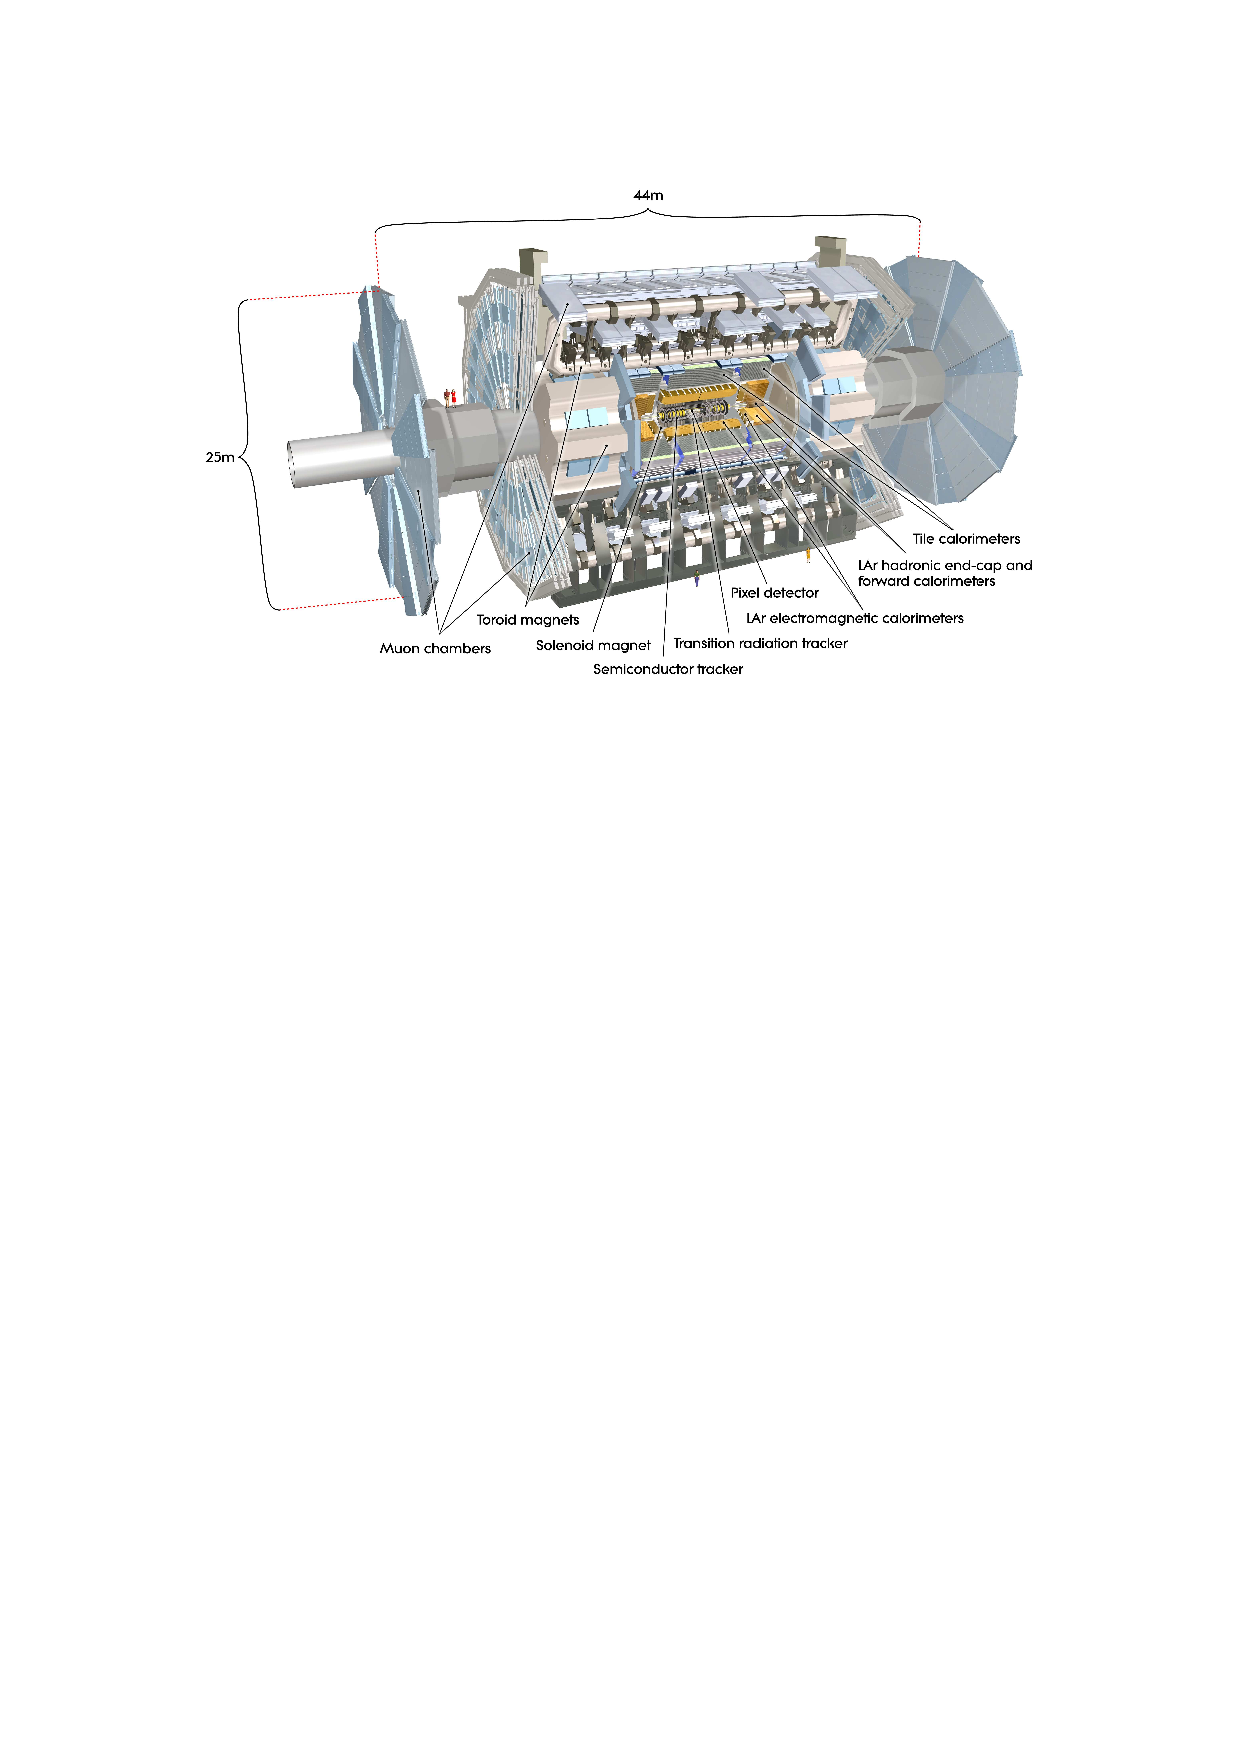
\includegraphics[width=.90\linewidth]{figures/atlas/detector.pdf}
\caption{Diagram of the \ac{ATLAS} detector, with subsystems and magnets identified.}
\label{fig:detector}
\end{figure}
\end{centering}

\section{Coordinate System Used in the \ac{ATLAS} Detector}
\label{sec:coords}

The \ac{ATLAS} detector is centered around the $pp$ collision point, and is built radially out from the beam pipe, maintaining as much rotational symmetry around the beam pipe as possible. It is also symmetric in the forward-backward directions. A coordinate system using the collision point as the origin is used, with the beam line defining the $z$-axis in the counter-clockwise direction. The positive $x$ direction is defined as pointing to the center of the \ac{LHC} ring, while the positive $y$ direction points upwards. For ease of reference, the side of the detector in the positive-$z$ direction is referred to as the A side, and the other side is referred to as the C side. 

Because of the cylindrical design of the detector, angular coordinates are often used. The azimuthal angle $\phi$ defines the angle around the beam pipe and the polar angle $\theta$ defines the angle from the beam axis ($z$). However, a transformation of the polar angle called pseudorapidity ($\eta$) is used more often, and is defined as 

\begin{equation}
\eta = - \mathrm{ln} [ \mathrm{tan} \frac{\theta}{2} ]. 
\end{equation}

$\eta$ is used because the particle distribution from \ac{LHC} collisions is roughly uniform in this variable. Building on this definition, angular distance between objects is typically defined as

\begin{equation}
\Delta R = \sqrt{\Delta\eta^2 + \Delta\phi^2}. 
\end{equation}

Often variables are defined purely in the transverse plane, which is indicated by a subscripted $T$, as in $p_T$, which gives an object's transverse momentum. 

%------------------------------------------------

\section{The Inner Detector}
\label{sec:ID}

The \acf{ID} is used for the measurement of tracks, estimates of the paths charged particles take as they travel through the detector. Collisions in the detector produce about 1000 particles, so identifying and differentiating all the tracks resulting from a collision is challenging. 

The \ac{ID} consists of three separate subdetectors, each of which has multiple layers capable of producing an electrical signal, called a \textit{hit}, when a charged particle travels through its active material. \ac{ATLAS} tracking software considers all these hits and forms tracks, with the goal of minimizing fake tracks due to random noise and maximizing the efficiency of identifying a real particle. Some details of this procedure are discussed in \autoref{sec:NN}. The full \ac{ID} can be seen in \autoref{fig:ID}, while a schematic in \autoref{fig:IDeta} shows more detail on the placement of each layer.

\begin{centering}
\begin{figure}[bth]
\myfloatalign
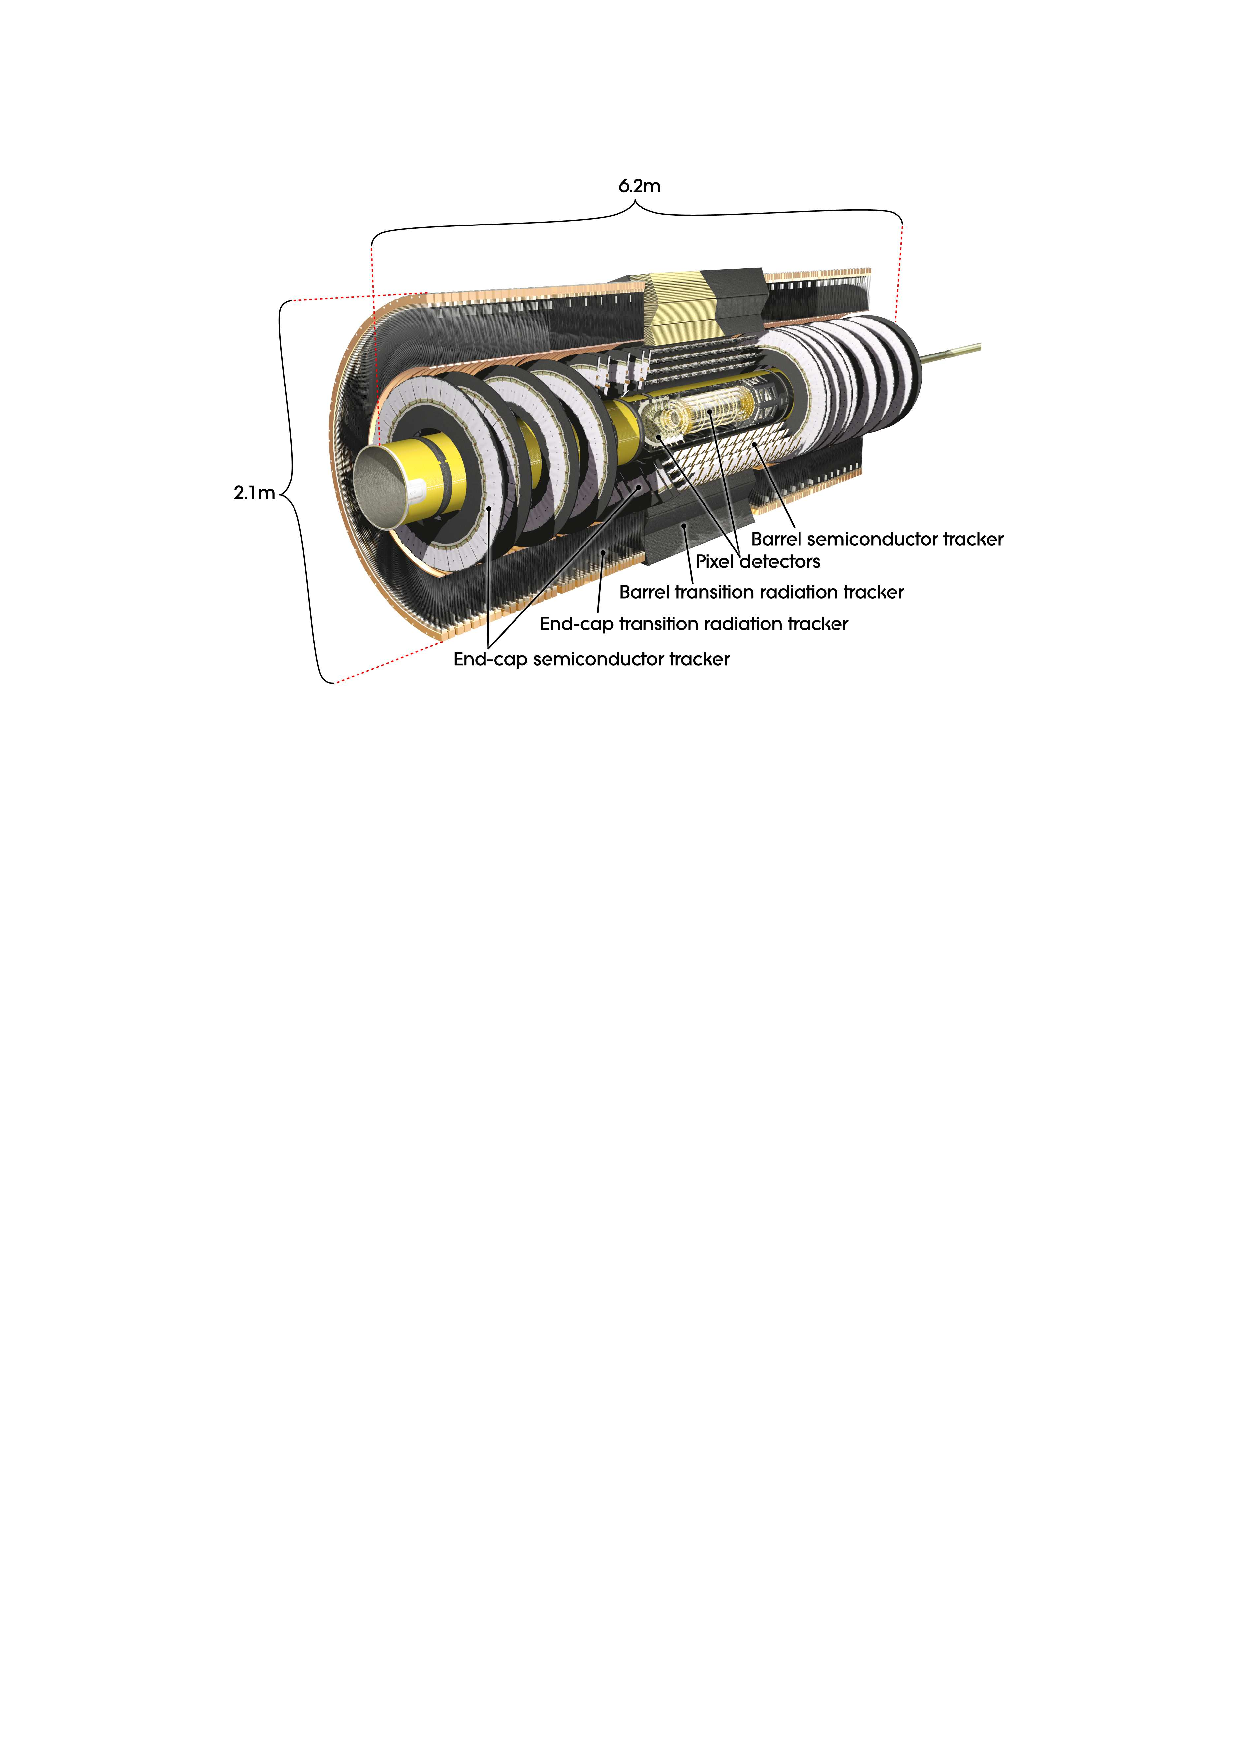
\includegraphics[width=.90\linewidth]{figures/atlas/innerdetector.pdf}
\caption{Diagram of the \ac{ATLAS} Inner Detector, containing the Pixel, SCT, and TRT subsystems.}
\label{fig:ID}
\end{figure}
\end{centering}

\begin{centering}
\begin{figure}[bth]
\myfloatalign
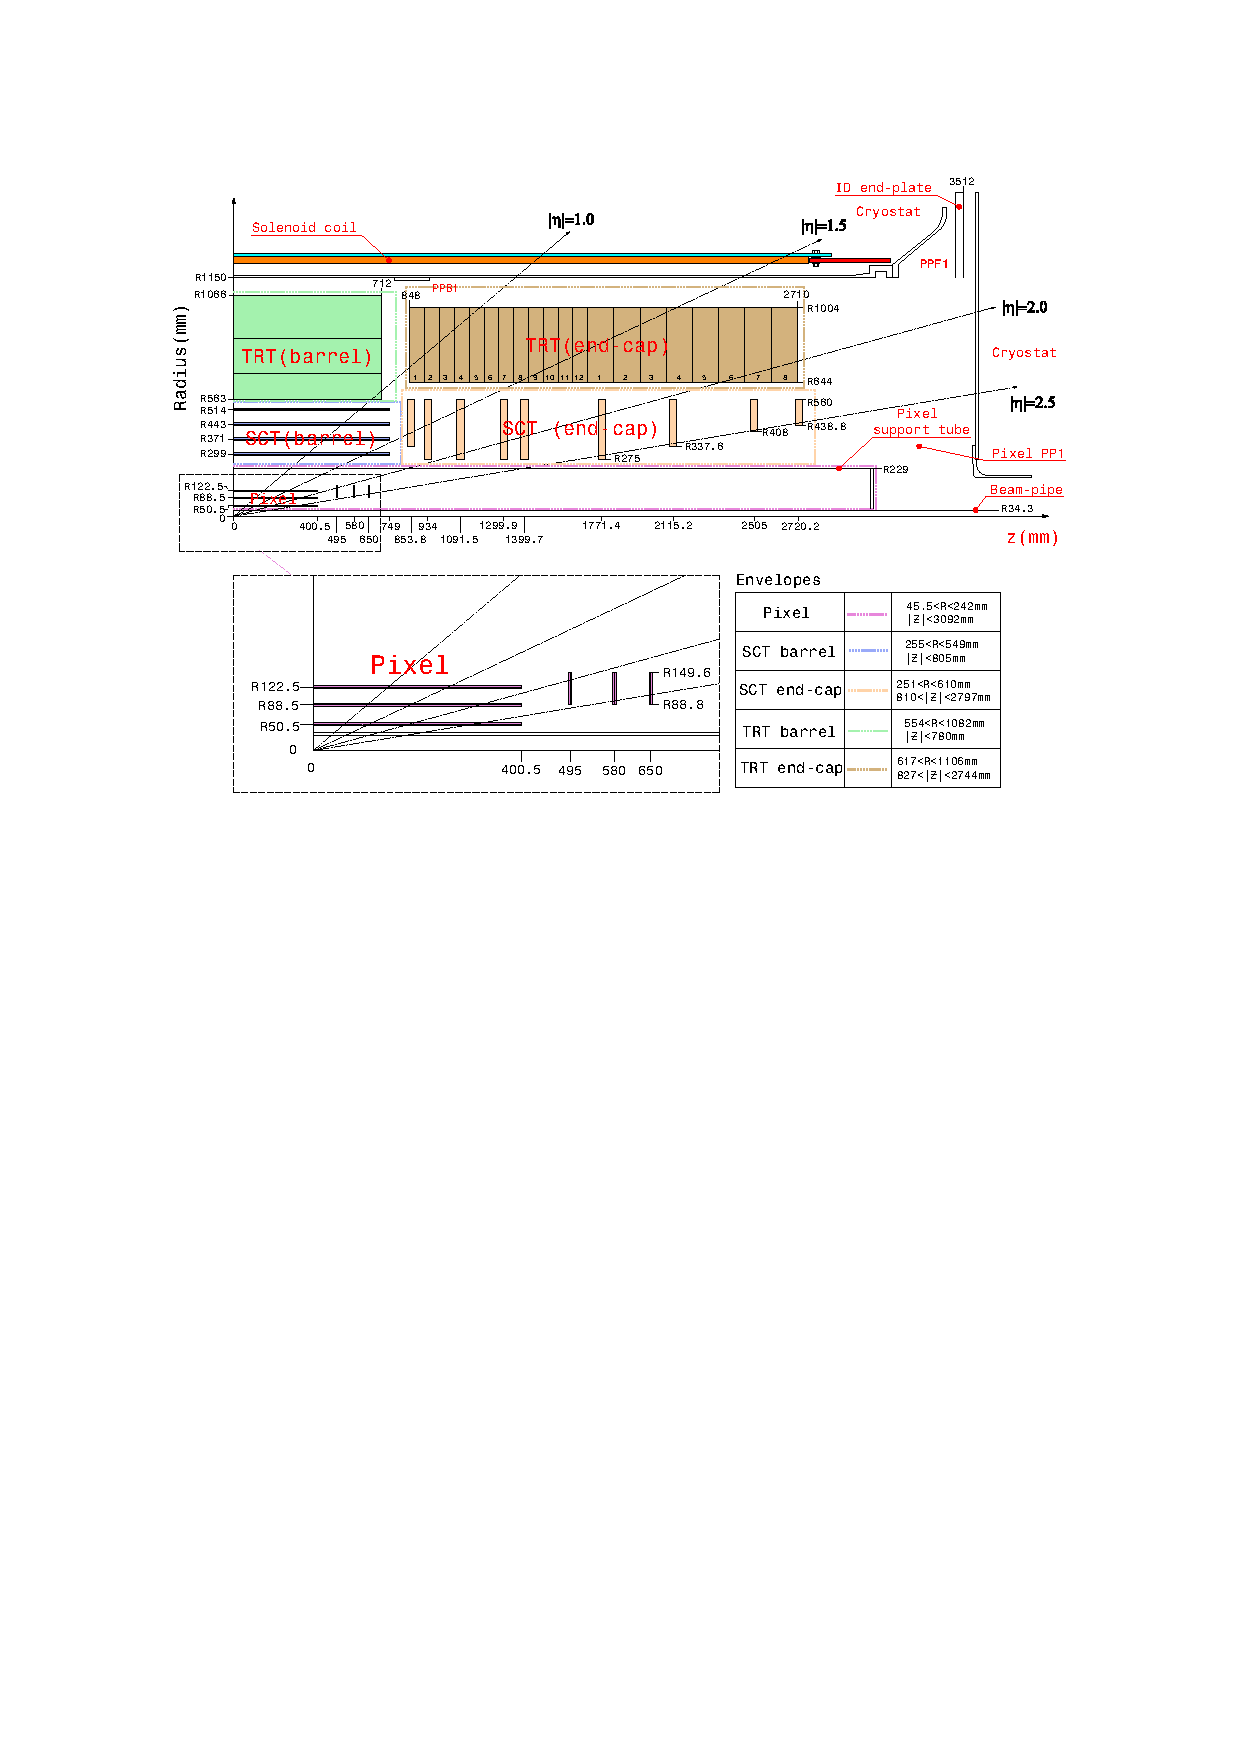
\includegraphics[width=.90\linewidth]{figures/atlas/ideta.pdf}
\caption{Diagram of one-quarter of the \ac{ATLAS} Inner Detector in the $R-z$ plane, with lines drawn to indicate various $\eta$ locations.}
\label{fig:IDeta}
\end{figure}
\end{centering}

\subsection{The Pixel Detector}

The pixel detector lies closest to the beam pipe of the \ac{LHC}, and has four layers comprising 92 million pixels. There are three standard layers, referred to as Layers 0-2 (L0, L1, L2), and an additional layer added for the 2015 data-taking, called the \ac{IBL}. 

\subsubsection{The Original Pixel Detector}

The Pixel Detector consists of high-precision silicon chip pixel modules, with 1744 in total, and each module is made up of 16 sensors each with its own read-out system. Each sensor is identical, containing 47232 pixels, which are typically each 50$\times$400 $\mu$m$^2$, though pixels at the edges of the sensors are slightly longer, at 50$\times$600 $\mu$m$^2$.  

As shown in \autoref{fig:IDeta}, the central $\eta$ region (barrel) is covered by three concentric cylindrical layers of sensors with radii of 50.5 mm, 88.5 mm, and 122.5 mm. In the higher $\eta$ region (endcap) is covered by a series of three disks positioned in the $x-y$ plane. Together, they give complete coverage out to $|\eta| = 2.5$, and a particle coming from the collision point will typically produce hits in three layers. 

The sensors are n-type silicon wafers with a voltage applied, and a passing charged particle produces thousands of electron-hole pairs inside the material, which drift in the electric field towards the mounted read-out system. A hit occurs when the resulting current becomes large enough to pass a threshold designed to suppress noise. A larger total charge deposit will result in the signal remaining over the threshold for a longer period of time. This \ac{ToT} is recorded along with the initial timing of the hit. This measurement is spatially accurate in the barrel (endcap) to 10 $\mu$m in the $R-\phi$ direction and 115 $\mu$m in the $z$ ($R$) direction.  

\subsubsection{Addition of the IBL}

In 2014, the \ac{IBL} was added to the Pixel Detector. This layer is placed directly on top of the beam pipe, inside barrel L0, providing a measurement of particles only 3.3 cm away from the interaction point. The \ac{IBL} consists of 14 overlapping staves, each containing 16 modules, the geometry of which can be seen in \autoref{fig:ibl_add}. These modules contain pixels measuring 50$\times$250 $\mu$m$^2$, and allow for particle detection in 90\% their area, as compared to the 70\% possible with the original pixel modules.

\begin{centering}
\begin{figure}[bth]
\myfloatalign
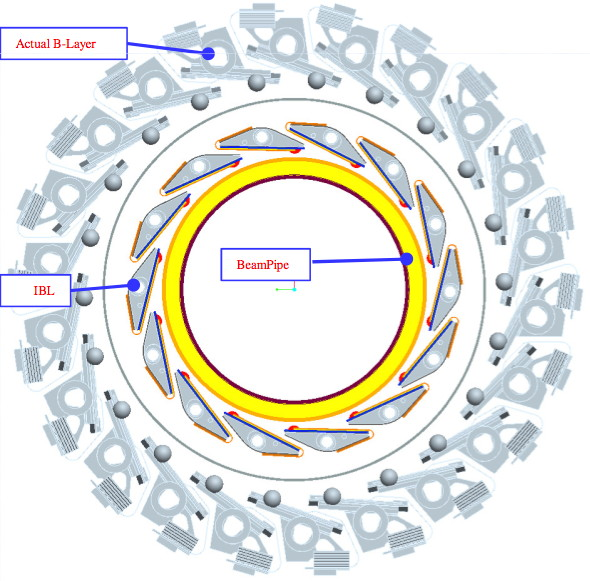
\includegraphics[width=.90\linewidth]{figures/atlas/IBL-other.png}
\caption{Diagram in the $x-y$ plane of the \ac{IBL} and the innermost layer of the pixel detector, L0 \cite{1201.5469}.}
\label{fig:ibl_add}
\end{figure}
\end{centering}

The \ac{IBL}'s addition provides greater precision for all track measurements, but it is especially useful for the detection of $B$ mesons, discussed in \autoref{sec:quarks}, whose lifetimes of about 1.5 ps allow them to travel as much as a few mm before decaying. These decays lead to secondary vertices in \ac{ATLAS} events. The location of the \ac{IBL} gives a measurement closer to these secondary vertices, increasing the probability that these vertices can be resolved. 

\subsection{The Silicon Microstrip Tracker}

The \ac{SCT} employs a similar technology to the Pixel Detector, with 15912 sensors and 6.3 million readout channels. Its main difference from the Pixel Detector is in the readout, which is performed by a series of 12 cm long strips with a width of 80 $\mu$m. These layers are paired, placed on top of one another at a small (40 mrad) angle to allow for position determination in the $\phi$ and $z$ directions. Together, these pairs of layers give four spatial measurements for each particle passing through the \ac{SCT}. In the barrel, these strips run parallel to the beam pipe, while in the endcap, they are arranged radially. These strips provide a hit resolution in the barrel (endcap) of 17 $\mu$m in the $R-\phi$ direction and 580 $\mu$m in the $z$ ($R$) direction. 

\subsection{The Transition Radiation Tracker}

The \ac{TRT} uses 4 mm diameter gas-filled tubes, each with a high voltage wire suspended along the center of the tube. The tubes run the length of the barrel, with a separate wire in the positive and negative $z$ direction. In the endcap, the tubes are arranged radially. In total, there are about 351,000 readout channels in the \ac{TRT}. This detector makes measurements only in the $R-\phi$ direction, where the resolution of each measurement is 130 $\mu$m, and coverage extends to $|\eta|=2.0$. Each particle typically creates about 36 hits as it passes through the \ac{TRT} barrel. 

Particles passing through the gas mixture of the \ac{TRT} ionize the gas, producing electrons which drift towards the wire due to a potential difference applied between it and the tube. In addition, particles passing through the \ac{TRT} produce radiation as they transition between materials, with larger amounts of radiation for lighter particles. This radiation produces high-threshold signals in the \ac{TRT} can be used to differentiate electrons from other heavier charged particles, such as pions. 


\section{The Calorimeters}
\label{sec:Calo}

Unlike the tracking detectors, which aim to take measurements of a particle with minimal alterations of its trajectory, the calorimeters measure the energy of objects by stopping them entirely. Calorimeters contain alternating layers of absorber, a material that causes incoming particles to shower into lower-energy decay products, and an active material, which detects passing particles, allowing for the reconstruction of these showers.

The \ac{ATLAS} calorimeters, which can be seen in \autoref{fig:calo}, provide coverage out to $|\eta| < 4.9$. High granularity electromagnetic measurements are made within $|\eta| < 2.5$. In this range, high-\pt electrons have nearly straight tracks, making momentum measurement through track curvature difficult, leaving the calorimeter as the primary energy measurement. The hadronic calorimeters, as well as the higher $|\eta|$ electromagnetic calorimeters, have a coarser granularity. 

\begin{centering}
\begin{figure}[bth]
\myfloatalign
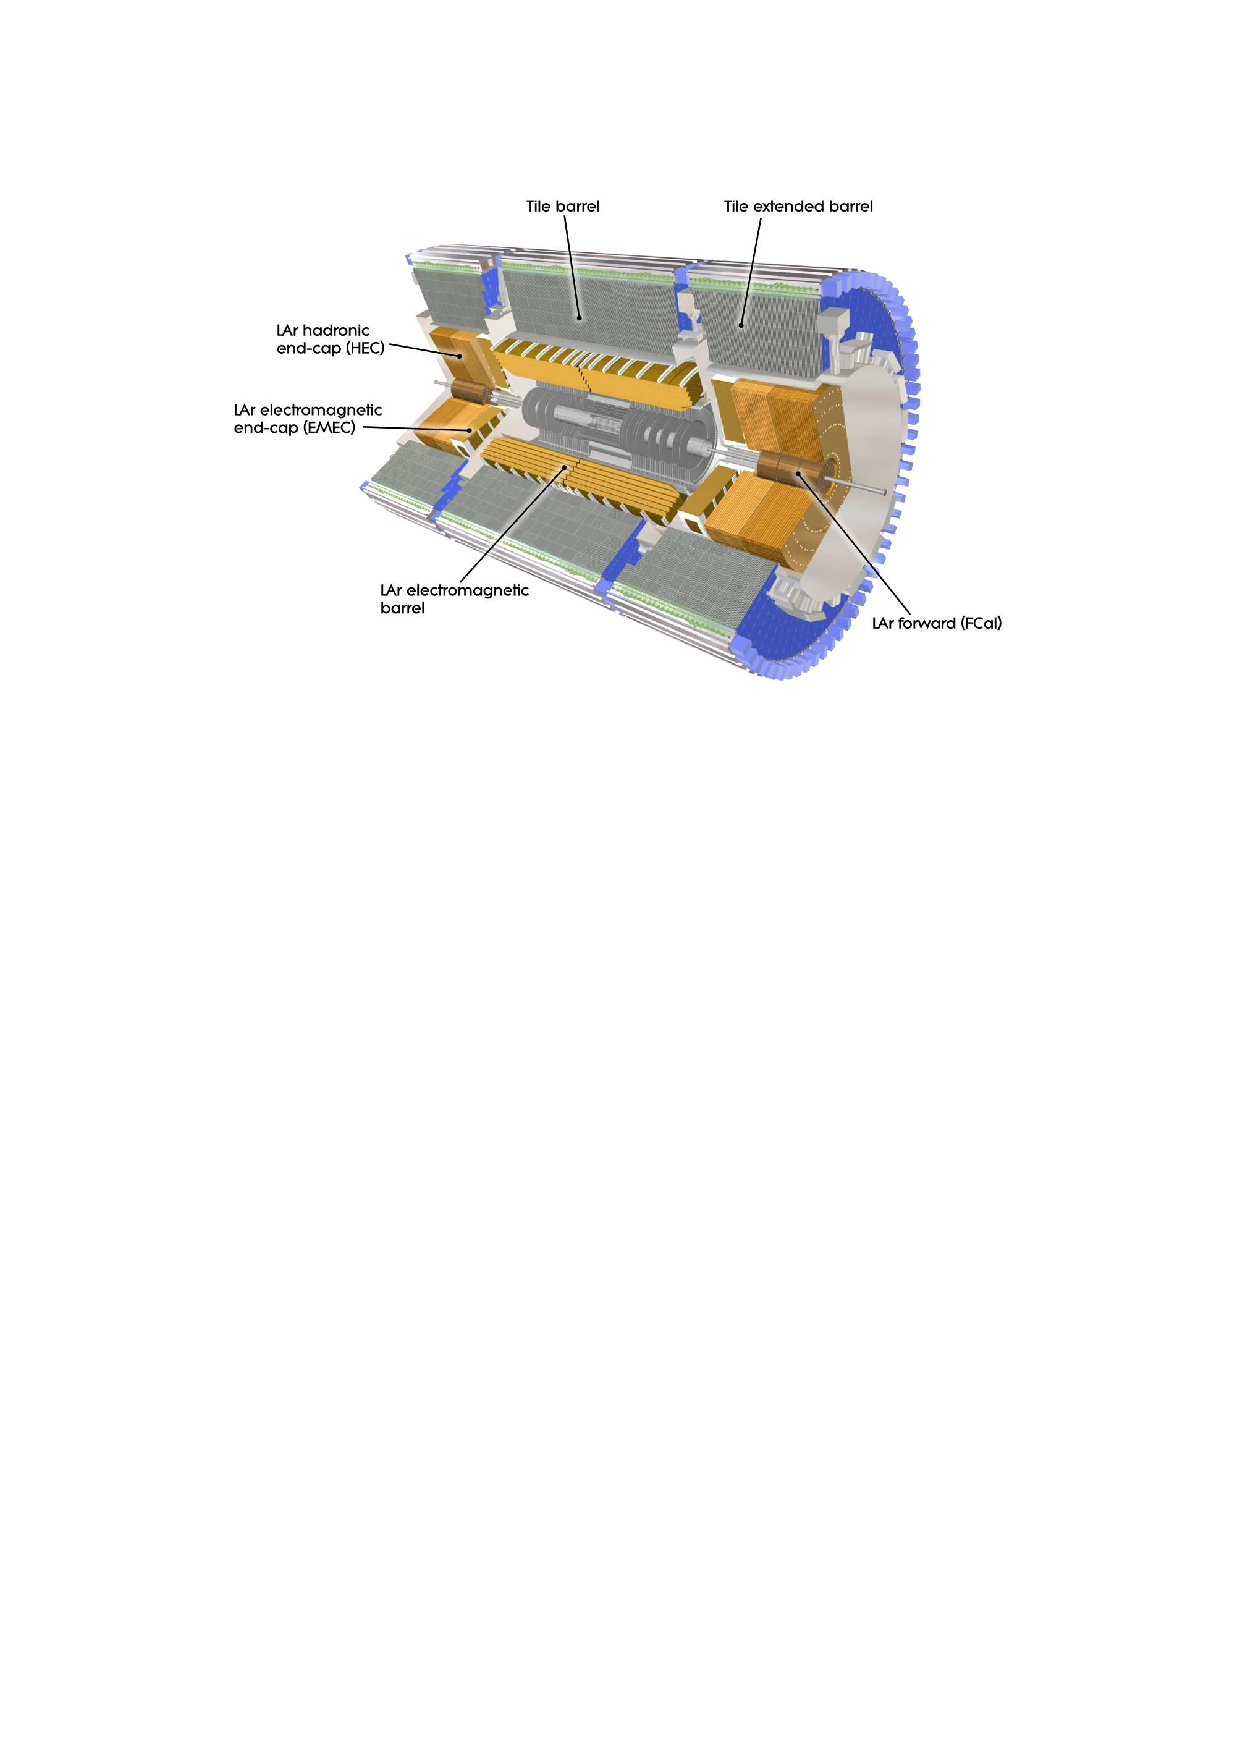
\includegraphics[width=.90\linewidth]{figures/atlas/calorimeters.pdf}
\caption{The calorimeter system of the \ac{ATLAS} detector.}
\label{fig:calo}
\end{figure}
\end{centering}

Besides measuring the energy of passing particles, another task of the calorimeter system is to limit punch-through to the \ac{MS}, described in \autoref{sec:MS}. All other particles must be fully stopped by the calorimeters to allow for clean signals from muons, and to measure the total energy of the particle. This requirement sets a minimum number of interaction lengths for each of the calorimeters. 

\paragraph{The LAr Electromagnetic Calorimeter} uses liquid argon as its active detector medium alternating with layers of lead acting as the absorber. Signals are read out with capacitively coupled copper plates. The layers are shaped like accordions, which allows for complete coverage with multiple layers of active material, three in central $\eta$ ($0<|\eta|<2.5$) and two at higher $\eta$ ($2.5 < |\eta| < 3.2$). \autoref{fig:calo_mod} shows the layout of a central $\eta$ module, including this accordion-like layering. At $|\eta| < 1.8$, an instrumented liquid argon presampler provides a measurement of energy lost prior to reaching the calorimeters. The total energy resolution for this detector is about 10\%/$sqrt{E}$, with an additional constant term of 0.2\%. 

\begin{centering}
\begin{figure}[!htb]
\myfloatalign
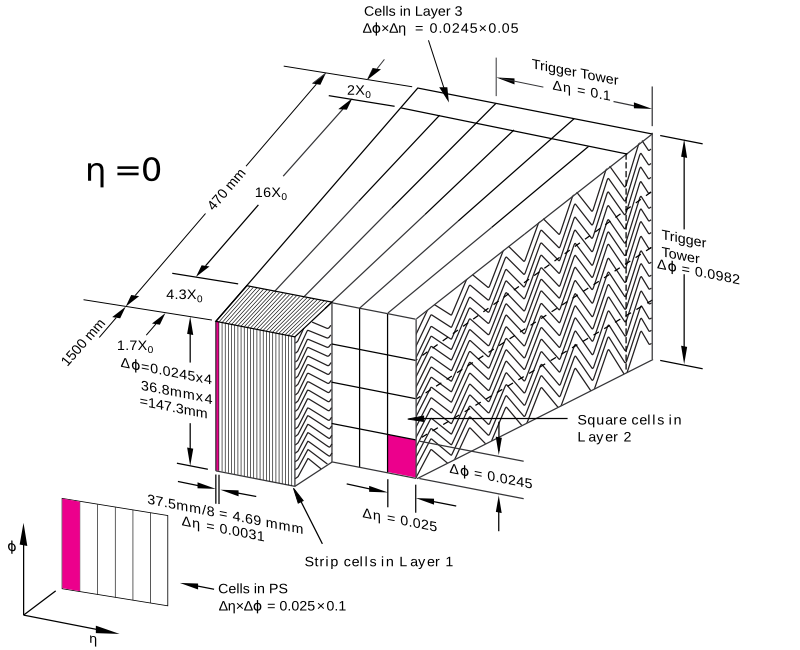
\includegraphics[width=.90\linewidth]{figures/atlas/LARG3-TDR-barrelM_samplings_presamp_new.png}
\caption{Layout of the LAr calorimeter module at central $\eta$ \cite{PERF-2007-01}.}
\label{fig:calo_mod}
\end{figure}
\end{centering}

\paragraph{The Tile Calorimeter} is a hadronic calorimeter which surrounds the LAr Calorimeter. It uses layers of steel as its absorber with scintillating tiles as the active material between them, which are read out by photomultiplier tubes. The Tile Calorimeter covers $|\eta| < 1.7$ with a typical energy resolution of about 50\%/$sqrt{E}$ with a constant term of 5\%. 

\paragraph{The LAr Hadronic Endcap Calorimeter} covers the hadronic calorimetery for higher $\eta$. It uses liquid argon active material and copper plate absorbers, resulting in an energy resolution of approximately 70\%/$sqrt{E}$ with a constant term of 5\%. This calorimeter covers $1.5 < |\eta| < 3.2$, overlapping with the hadronic calorimeters in either direction of its $\eta$ range. 

\paragraph{The FCal} or forward calorimeter provides electromagnetic and hadronic coverage at very high $\eta$ ($3.1 < |\eta| < 4.9$). This calorimeter also uses liquid argon as its active material, and uses copper-tungsten as the absorber. Its energy resolution is about 70\%/$sqrt{E}$ with a constant term of 3\%.

\section{The Muon Spectrometer}
\label{sec:MS}

The \acf{MS} measures charged particles that penetrate the calorimeter system. Because the calorimeters are designed to completely absorb electrons, photons, and hadrons, the \ac{MS} mainly detects muons, which pass through the calorimeter with very little loss of energy. The goal of the \ac{MS} is to give a high-precision measurement of these muons, and also to be able to quickly identify events with muons for the sake of triggering, discussed in \autoref{sec:Trigger}. The layout of the \ac{MS} can be seen in Figures~\ref{fig:muon_xy} and~\ref{fig:muon_rz}. Muons can be measured for all $|\eta|$<2.7, and they can be triggered on for $|\eta|$<2.4. The entire system is about 24 m tall and 40 m long. 

\begin{centering}
\begin{figure}[bth]
\myfloatalign
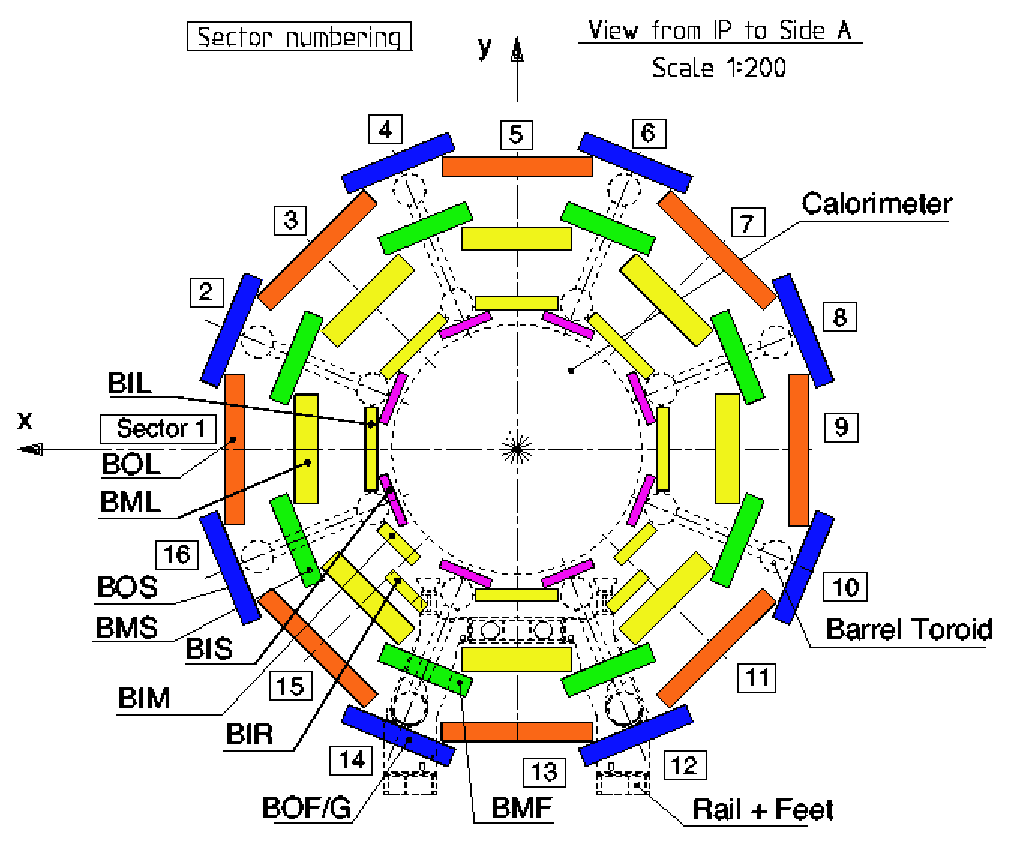
\includegraphics[width=.90\linewidth]{figures/atlas/Muon_sector_numbering.eps}
\caption{An $x$-$y$ view of the \ac{MS}. The three barrel layers are visible, as well as the overlapping, differently sized chambers. The outer layer of the \ac{MS} is about 20m in diameter.}
\label{fig:muon_xy}
\end{figure}
\end{centering}

\begin{centering}
\begin{figure}[bth]
\myfloatalign
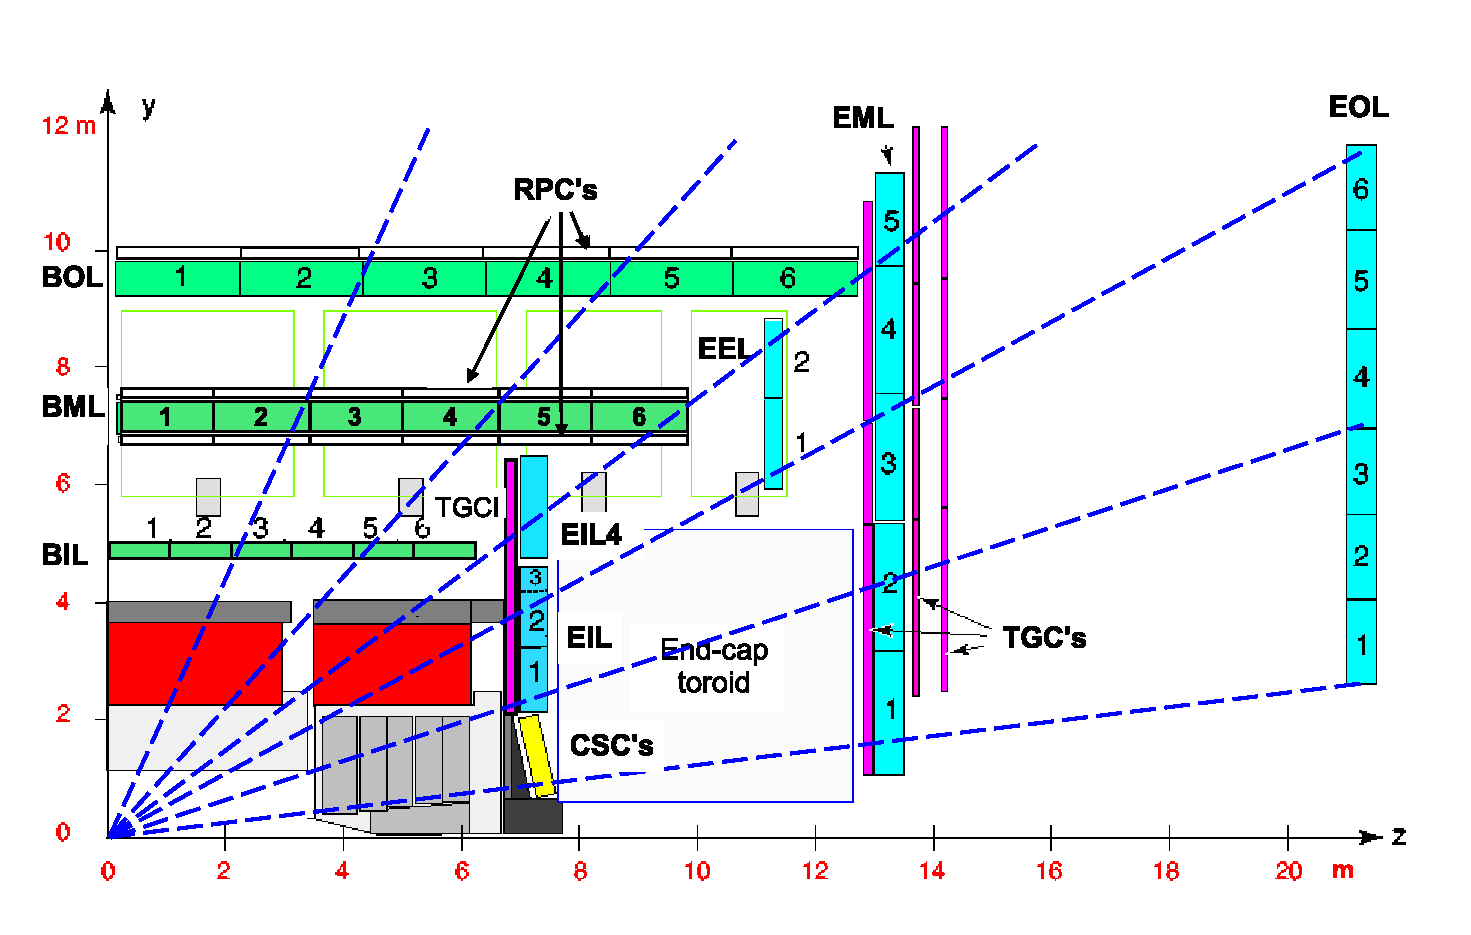
\includegraphics[width=.90\linewidth]{figures/atlas/Muon_rz_large_sect_6.eps}
\caption{An $r$-$z$ view of the \ac{MS}. The three layers of the barrel and endcap \ac{MS} are visible.}
\label{fig:muon_rz}
\end{figure}
\end{centering}

To achieve these goals, the \ac{MS} has several subsystems. The system responsible for precision measurement is called the \acfp{MDT}. This subdetector consists of chambers of three to eight layers of tubes, with three layers of chambers covering both the barrel and endcap regions. In the barrel, these chambers are arranged in layers concentric cylinders with small overlaps between adjacent chambers. The chambers are oriented such that the drift tubes are parallel to the beam line. In the endcap, the chambers form disks with drift tubes approximately aligned in the $R$ direction. 

The tubes each contain an Ar/CO$_2$ gas mixture and a single high voltage wire which runs at its center along its length. Charged particles excite the gas as they pass through it, producing electrons which drift towards the high voltage wire. The resulting electric signal is read out, and the magnitude and timing of the signals are both used to differentiate particle traces from noise. 

Though very effective at giving a precise measurement, the \acp{MDT} have two shortcomings. The first is that the measurement is only precise in the direction perpendicular to the tubes; in the direction parallel to them, the resolution is not much better than the length of the drift tube, which are typically several meters long. The resolution in the perpendicular direction is about 35 $\mu$m with the combined measurement of all the tubes in a chamber. The second major shortcoming is that the \acp{MDT} are slow, with a maximum drift time of about 700 ns. 

The slow drift time means that muons from sequential collisions can appear in the same event, and that the signals from the \acp{MDT} are received too late to be used for triggering. To solve the former problem, another detector called the \acp{CSC} is used in high-rate regions of the \ac{MS}. This detector consists of multi-wire proportional chambers which have cathode strips on either side of the anode in orthogonal directions, providing a 40 $\mu$m resolution in one direction and 5mm resolution in the other. Their drift times are much shorter than those of the \acp{MDT}, at about 40 ns. They are placed in the forward region of the detector (2<$|\eta|$<2.7) where the incident particle rates are highest. 

To achieve responses fast enough to be used for triggering, \acp{RPC} and \acp{TGC} are used. These chambers both take less than 25 ns to produce a signal. The \acp{RPC} are used in the barrel and are made up of two high-resistance plastic plates with a gas mixture under an electric field between them. Passing particles ionize this gas, and the resulting signal is read out via metallic strips mounted to the plastic plates. The \acp{TGC} used in the endcap are a form of multi-wire proportional chambers, like the \acp{CSC}. Unlike the \acp{CSC}, the cathode is placed extremely close to the wires, speeding up its operation. 

The massive \ac{MS} is subject to deformations due to gravity and the magnetic field. To achieve a high precision alignment, these deformations are constantly monitored in each \ac{MDT} chamber with a set of four optical alignment rays, which give alignment information at the precision of <30 $\mu$m. In addition, a sag-adjustment system can use this information to re-align any wires that droop under gravity's pull. Lastly, the \ac{MS} can be aligned using the tracks made from hits it measures, discussed more in \autoref{sec:reco_muons}.

\section{The Magnet System}
\label{sec:magnets}

The \ac{ATLAS} magnet system consists of four superconducting magnets: an inner solenoid, a barrel toroid, and two endcap toroids. Collectively, they are 22m in diameter and 26m long, and their basic layout can be seen in \autoref{fig:magnets}.

\begin{centering}
\begin{figure}[bth]
\myfloatalign
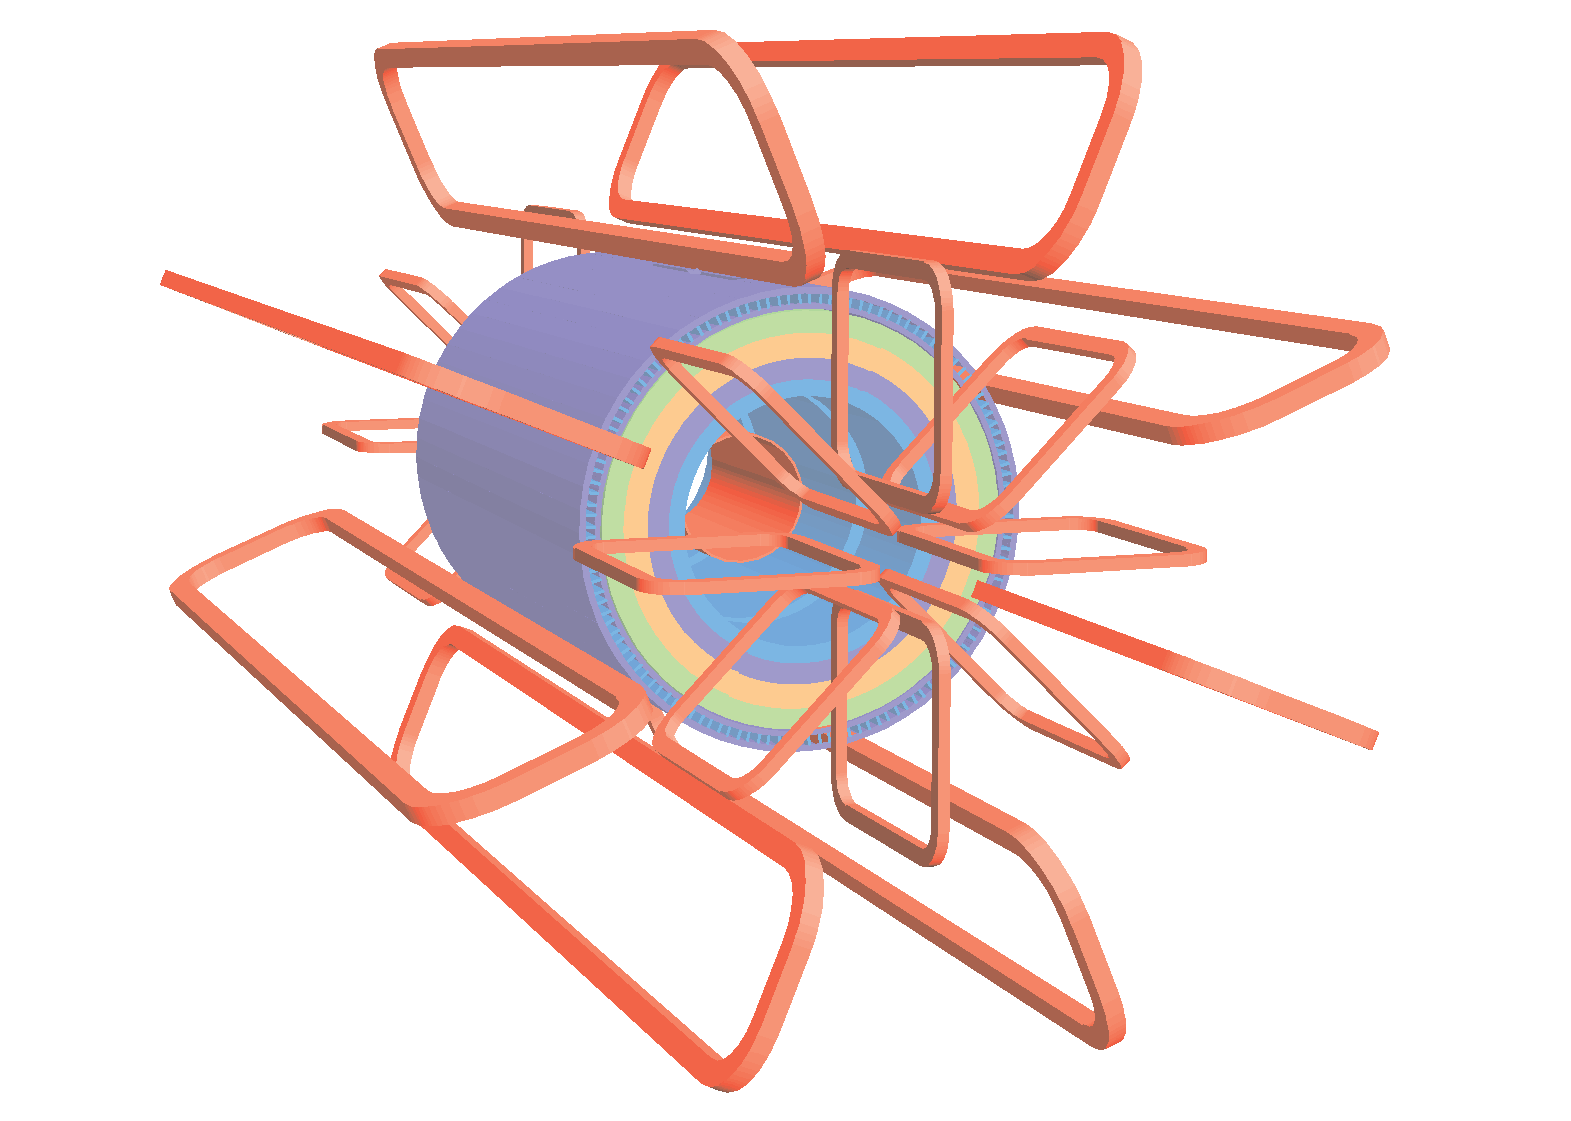
\includegraphics[width=.90\linewidth]{figures/atlas/ATLcoilGeom.eps}
\caption{The magnet system of the \ac{ATLAS} detector. The inner cylinder shows the solenoid which gives a uniform magnetic field in the \ac{ID}. Outside of that are the barrel and endcap toroids, which provide a non-uniform magnetic field for the \ac{MS}.}
\label{fig:magnets}
\end{figure}
\end{centering}

The solenoid is inside the calorimeter volume and provides a uniform 2T magnetic field for particles traveling through the \ac{ID}. This axial field causes the trajectories of charged particles to bend in the $x-y$ plane, and measurements of the curvature of these trajectories give the most accurate \pt measurement for many particles according to the equation

\begin{equation}
\pt = qB\rho 
\end{equation}

where $q$ is the charge of the particle, $B$ is the magnetic field in the $z$ direction, and $\rho$ is the radius of curvature. 

Because the solenoid is placed between the tracking system and the calorimeter, it is important that it interfere minimally with particles in order to allow the calorimeter to measure their full energies. The solenoid is placed inside the same vacuum chamber as the LAr calorimeter and is made of Al-stabilized NbTi superconductor with aluminum casing, giving it a total thickness of about 0.66 radiation lengths. 

The barrel toroid is outside the calorimeters and provides the magnetic field for the barrel \ac{MS}, which varies from 0.2–2.5T. The endcap toroids have a magnetic field range of 0.2-3.5T. All three toroid magnets are made with Al-stabilized Nb/Ti/Cu superconducting coils supported by Al-alloy struts. 

The magnets are cooled with liquid helium, and take up to a month to be brought down to operating temperatures, about 4.5 K. All magnets have cold masses surrounding them to absorb heat in the event of a quench. 

The $B$-field resulting from this magnet system can be seen in \autoref{fig:bfield}. The plot on top demonstrates the relatively constant field rate within the barrel which drops steeply at $|z|$=2. The bottom plot shows the field integral in the \acp{MDT} as a function of $|\eta|$, demonstrating the good coverage out to $|\eta|$<2.6 excluding a transition region between the barrel and endcap, where the field changes rapidly, making precise \pt construction difficult. 

\begin{centering}
\begin{figure}[!htb]
\myfloatalign
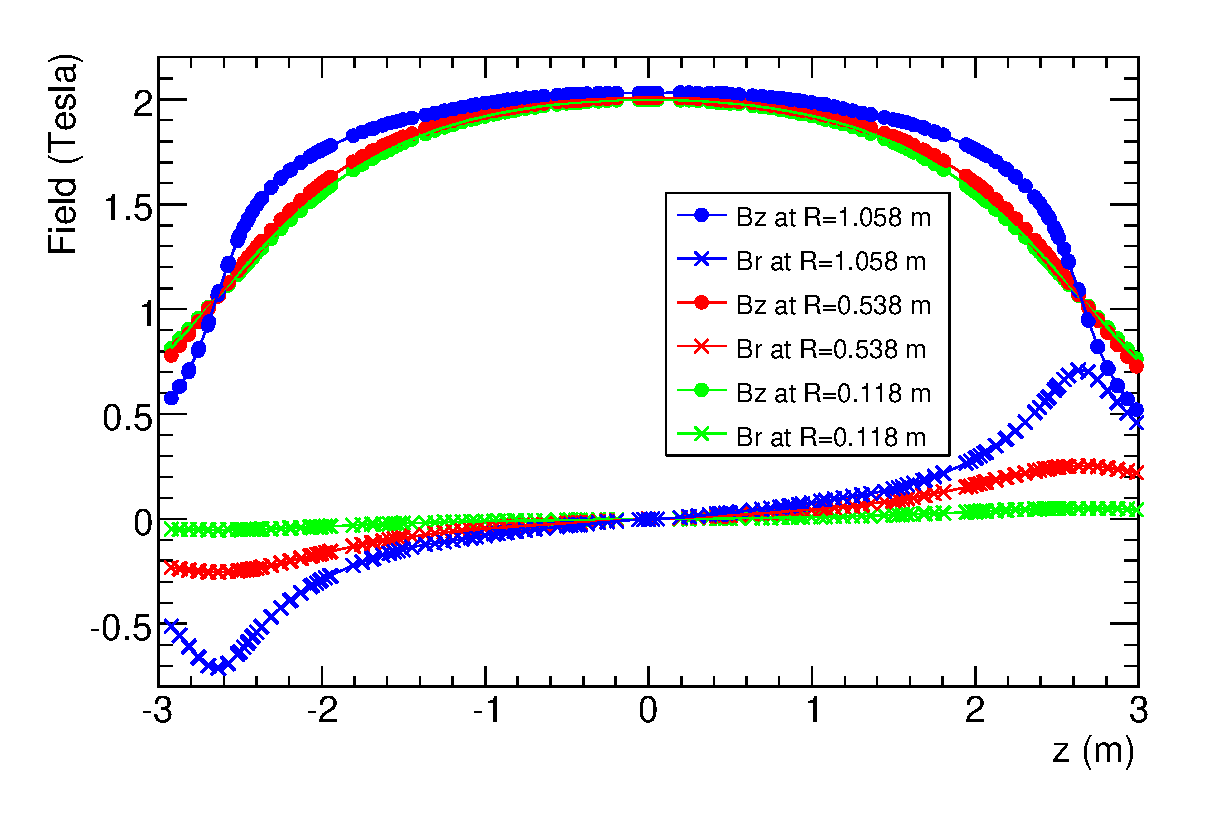
\includegraphics[width=.90\linewidth]{figures/atlas/solMeasB.eps}
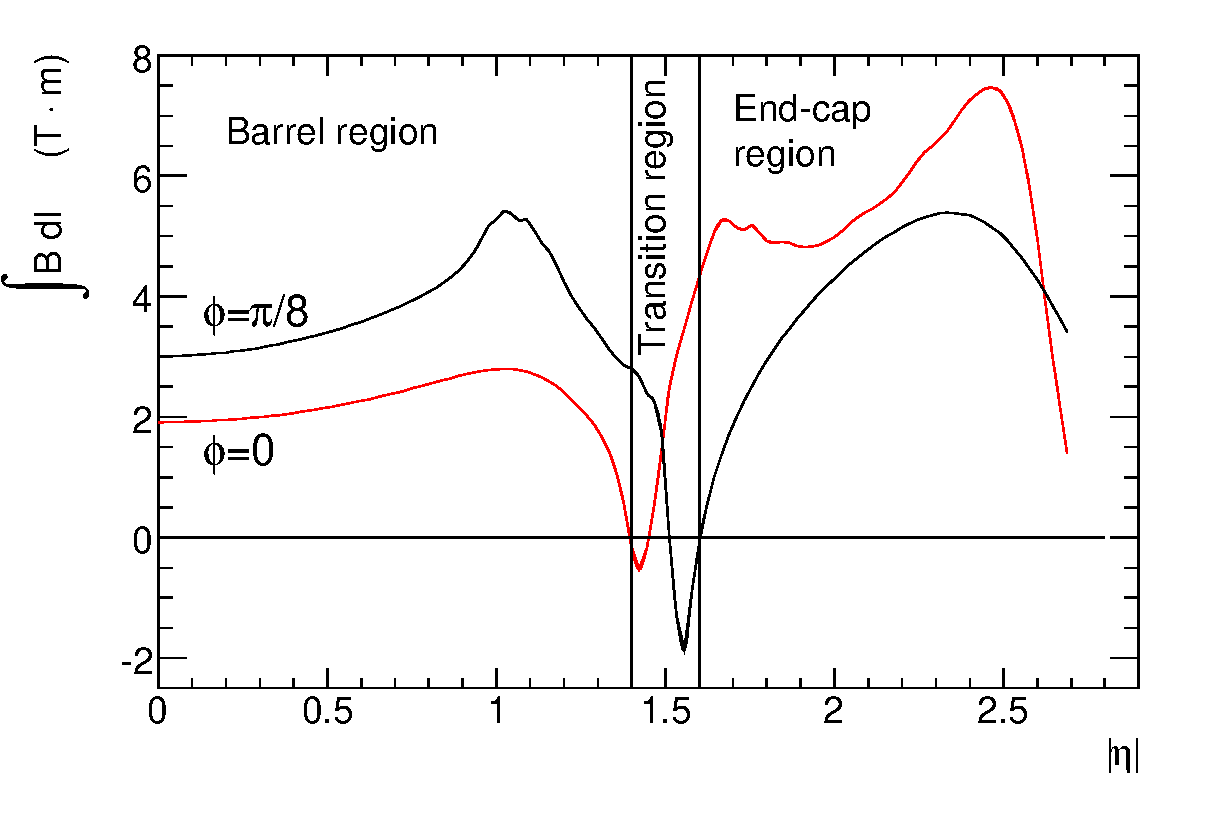
\includegraphics[width=.90\linewidth]{figures/atlas/IBdl.eps}
\caption{Plots of the magnetic field within the \ac{ATLAS} detector. Top is the field (broken into its $R$ and $z$ components) as a function of $z$ for several different values of $R$. Bottom is the field integral through the \acp{MDT} as a function of $|\eta|$ for two different $\phi$ values. }
\label{fig:bfield}
\end{figure}
\end{centering}

\section{The Trigger System and Data Acquisition}
\label{sec:Trigger}

The \ac{LHC} provides proton bunch crossings every 25 ns, and each of these events contains about one MB of data, corresponding to 40 TB/s\footnote{ This number is actually an overestimate, as not all bunches are filled due to the gaps produced by the \ac{LHC}'s injector complex, discussed in \autoref{sec:lhc_inj}.}, a completely unmanageable amount of data. In addition to this concern, many of \ac{ATLAS}'s subdetectors like the Pixel Detector, the LAr Calorimeter, and \acp{MDT} take much longer than 25 ns to read out, making keeping up with the bunch crossing rate impossible. To reduce the total data read out and allow for selective reading out of the slower detectors' buffers, a triggering system is used. 

The trigger system uses fast detectors to get a coarse picture of an event's topology, which is then compared to a trigger menu, which lists the types of events that are interesting enough to keep. Overall, the trigger system reduces the 40 million events a second to about 1000 to be fully read out from the \ac{ATLAS} detector. 

This filtering of events is done in two steps: the \ac{L1} trigger is implemented in hardware and reduces the initial 40MHz to 100kHz, while the \ac{HLT} is implemented in software, further reducing the rate to 1kHz \cite{ATL-DAQ-PUB-2016-001}. The \ac{L1} trigger uses coarse granularity information from the fast read-out subdetectors: the calorimeters, the \acp{RPC} and \acp{TGC}. 

The coarse grained calorimeter information used for the \ac{L1} trigger decision is referred to as \ac{L1Calo} and uses information from all calorimeter systems. \ac{L1Calo} is responsible for all triggers excluding muons, meaning it must be capable of identifying a large number of different objects and event topologies, including high-\pt objects, \met, and large amounts of hadronic energy. The trigger can also identify isolated objects, objects with very few calorimeter deposits from other objects near them.

For muon triggers, the trigger algorithm looks for patterns of hits from the \ac{RPC} and \ac{TGC} that are consistent with high-\pt muons with origins at the interaction point. 

An example of the \ac{L1} trigger rates for different types of events can be seen in \autoref{fig:l1_rates} for one run in July 2016. The common features to all rates are due to \ac{LHC} luminosity changes, deadtimes due to detector inefficiency, and adjustment of trigger rates to optimize bandwidth.

\begin{centering}
\begin{figure}[!hbt]
\myfloatalign
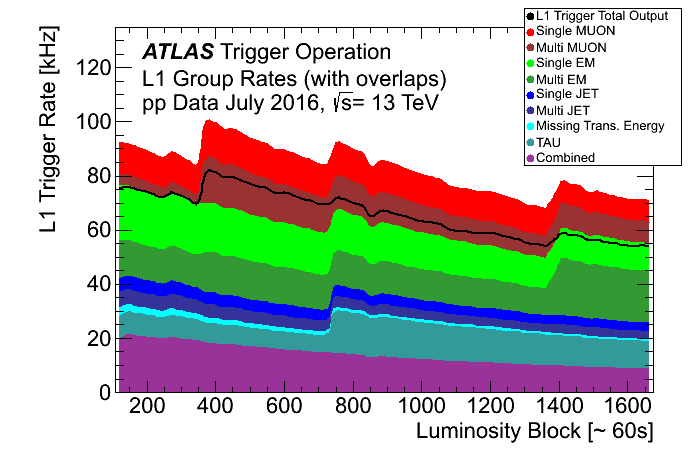
\includegraphics[width=.90\linewidth]{figures/atlas/Time_L1GroupRate_Stack_2016_07.png}
\caption{\ac{L1} trigger rates for for a run in July 2016 as a function of luminosity block, an approximately 60-second long period of data-taking. The total rate is lower than the combined stack because of overlapping triggers.}
\label{fig:l1_rates}
\end{figure}
\end{centering}

%The outputs from the different calorimeters and the \ac{MS} can also be combined with a system called \ac{L1Topo}. Using this, triggers can require more complex topologies, and can suppress backgrounds by as much as a factor of two. 

All of this information is analyzed by the \ac{CTP}, which uses a trigger menu identifying all types of events to be kept to return a trigger decision. Due to the limited size of detector buffers, the event must be processed in about 2.5 $\mu$s. This ensures that the information to be read out has not yet been overwritten when the trigger decision is made. This decision is passed to the \ac{TTC}, which communicates with all subdetectors. Upon receiving a \ac{L1} trigger, the subdetectors read out all the information they've stored about the event and place it on their \acp{ROB}.

The \ac{HLT} takes the data from particular \acp{RoI}, areas containing interesting objects that caused the \ac{L1} trigger. With a more complete picture of the hits observed by the detector, tracks are formed, and the \ac{HLT} can use all of this information to determine whether or not the event is still interesting enough to keep. This process has its own trigger menu with dedicated \ac{L1} seeds for each item. \ac{HLT} triggers typically have slightly higher thresholds than their corresponding \ac{L1} triggers to ensure that events that would pass the \ac{HLT} requirements are very likely to have passed the \ac{L1} requirements. \autoref{fig:hlt_rates} shows the \ac{HLT} rates for the same run in July. In addition to the event types seen in \autoref{fig:l1_rates}, the \ac{HLT} can also identify events with $b$-jets, differentiate between electrons and photons, and identify events interesting for B-physics. 

\begin{centering}
\begin{figure}[!hbt]
\myfloatalign
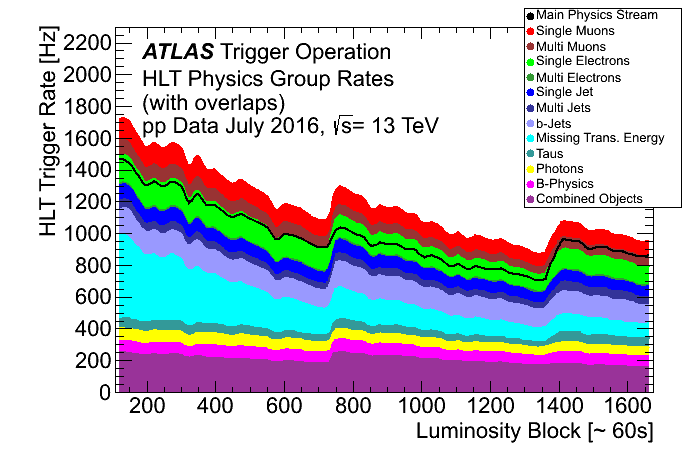
\includegraphics[width=.90\linewidth]{figures/atlas/Time_HLTGroupRate_Stack_2016_07.png}
\caption{\ac{HLT} trigger rates for for a run in July 2016 as a function of luminosity block, an approximately 60-second long period of data-taking. The total rate is lower than the combined stack because of overlapping triggers.}
\label{fig:hlt_rates}
\end{figure}
\end{centering}


Events passing the \ac{HLT} trigger are written to disk to be analyzed. An example of the total trigger efficiency for single electron triggers is shown in \autoref{fig:trig_el_eff}. %Trigger efficiencies can be taken directly from \ac{MC}, and are measured in data via a method called tag-and-probe, the main principles of which are discussed in \autoref{sec:bg-fake}.

Events types that occur very frequently, such that it would require too much of the total trigger bandwidth to record all events passing a given threshold, are prescaled. Events passing these triggers are only recorded a fraction of the time, and these prescaling rates are used to weight events passing these triggers when they are analyzed. For example, the lowest unprescaled single electron trigger in 2016 data-taking required an electron with \pt of 60 \gev. A trigger requiring electrons with \pt of only 10 \gev~also exists, but only one in ten events passing this trigger is recorded. 

\begin{centering}
\begin{figure}[!hbt]
\myfloatalign
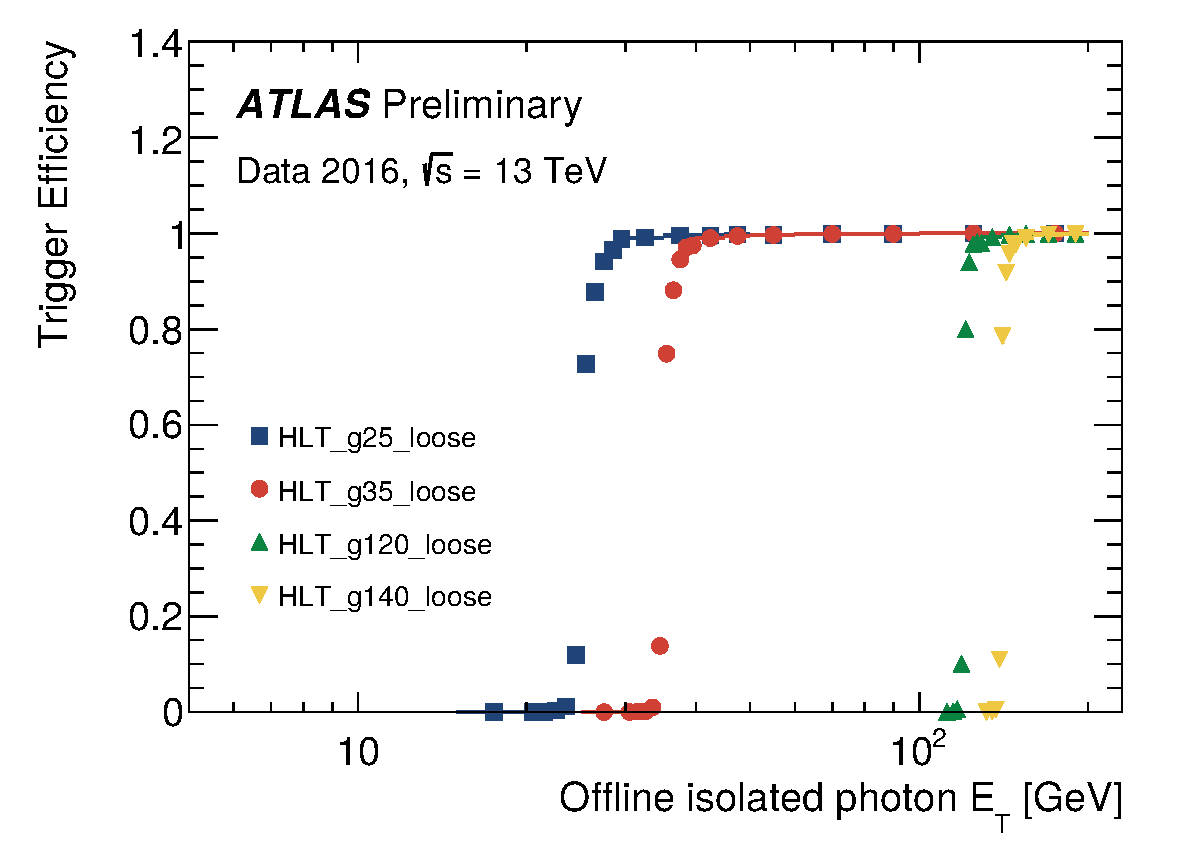
\includegraphics[width=.90\linewidth]{figures/atlas/plot_Combined_Pt_LOGaxis_Et_log_25l_35l_120l_140l.pdf}
\caption{Photon trigger efficiency as a function of \et for four different \ac{HLT} triggers with photon \pt requirements of 25, 35, 120, and 140 \gev~\cite{egamma_trig}.}
\label{fig:trig_el_eff}
\end{figure}
\end{centering}


\section{Monte Carlo Event Generation}
\label{sec:MC_gen}

The complex events of the \ac{LHC} are difficult to model, but modeling them is crucial to analyzers' understanding of \ac{SM} backgrounds and potential signals. To simplify the modeling process, particle interactions are broken down into very small steps, each with associated probabilities of various outcomes. This modeling method is called \acf{MC}, and, at the \ac{LHC} it is broken into several larger steps which are each handled by different software. 

The first step, discussed in \autoref{sec:pp_collisions}, is to determine the energies of the initial particles in a collision, which are provided by several different \ac{PDF} sets. These distributions come from experimental measurements, though there is some variation between different sets. Three different sets are used in this analysis: NNPDF2.3LO \cite{Ball:2012cx} and NLO CT10 \cite{Lai:2010vv} for background and signal processes, and MSTW 2008 \cite{0901.0002} for pile-up events, discussed more in \autoref{sec:pileup}. 

With the initial states of the constituents of the protons described by these probabilistic models, the next step is to model the hard scattering process resulting from the interaction of two of these particles. This is accomplished by a generator, which calculates the cross-sections of the Feynman diagrams of a given process. In particular, these generators typically produce matrix elements, which describe the probability to go from an initial to final state via a hard scattering, including the kinematic properties of the final state. The generator uses these matrix elements to assign one of these hard scattering final states to each event. These hard scattering outputs are then passed to the next step, where parton showering, hadronization, and final and initial state radiation can occur.

Because these matrix elements must be calculated for each event's specific kinematic properties, it can be very computationally intensive, especially when the calculations are performed at very high order. To save computational time, matrix elements are sometimes calculated at a lower order, and later, the total cross-section for a given process can be calculated at a higher order and used to scale the overall number of events generated for the process. These calculations can also be tuned, varying parameters in the generation to create outputs that most closely match experimental data. 
  
%In some cases, this can mean that a tune might include values for certain physical quantities that are different from their measured values because this configuration ultimately produces a result more similar to data. 

Examples of generators include {\sc MadGraph5\_aMC@NLO} \cite{Alwall:2014hca}, {\sc Powheg Box} \cite{PowhegBOX1,PowhegBOX2,PowhegBOX3}, and \sherpa~\cite{sherpa}. Each has different strengths and is used to describe processes that best match those strengths. {\sc Powheg Box}, for example, cannot perform its own parton showering, and must be interfaced with another generator, typically {\sc Pythia} \cite{Sjostrand:2006za}, in order to describe any physics processes beyond the hard scattering, which can cause discontinuities in its predictions for large numbers of partons. However, it can calculate matrix elements at \ac{NLO}, giving it an advantage in calculating some complex processes. \sherpa performs its own parton showering, but in most cases calculates its matrix elements at \ac{LO}. The main advantage of {\sc MadGraph5\_aMC@NLO}, which must also be interfaced with another generator (typically {\sc Pythia}) to perform parton showering, is its simple user interface. Instead of designating specific processes to be generated, it allows users to specify a final state to be generated, and all processes capable of producing that state will be included.

Once the final state particles of the hard interaction and showering have been calculated, the pile-up of the \ac{LHC} (described in \autoref{sec:pileup}) must be accounted for. Events called \textit{minimum bias} are generated to match the overall production of the \ac{LHC} collisions, with no preselection. These events are overlaid on the original hard scatter to produce a more realistic representation of the many simultaneous interactions observed in the \ac{ATLAS} detector.

This collection of particles must then be translated into signals in the detector. Their trajectories in the magnetic fields of the detector, their interactions in each layer, and the way these interactions deposit charge in each subdetector are modeled in software called {\sc GEANT4}~\cite{Agostinelli:2002hh}. In this software, every piece of the \ac{ATLAS} detector is modeled, including the magnetic field and the many different materials. Particles then follow trajectories through the simulated detector and interact with the different materials based on several preprogrammed options for each material. For example a photon traveling through a material could continue along its trajectory, convert into a positron-electron pair, or deposit energy. As it crosses into a new material, a new set of options opens up for interactions. The particle is tracked until all of its energy is lost or it exits the geometry of the simulation.

The model of the detector used for this process is iteratively perfected by comparing data to \ac{MC}. \autoref{fig:geant} shows an example of a discrepancy between the simulation and observed data in the number of secondary vertices in a pixel module, which should correspond to the amount of material in the area. Observations of discrepancies like this can be used to correct the materials in the simulation. 

\begin{centering}
\begin{figure}[!hbt]
\myfloatalign
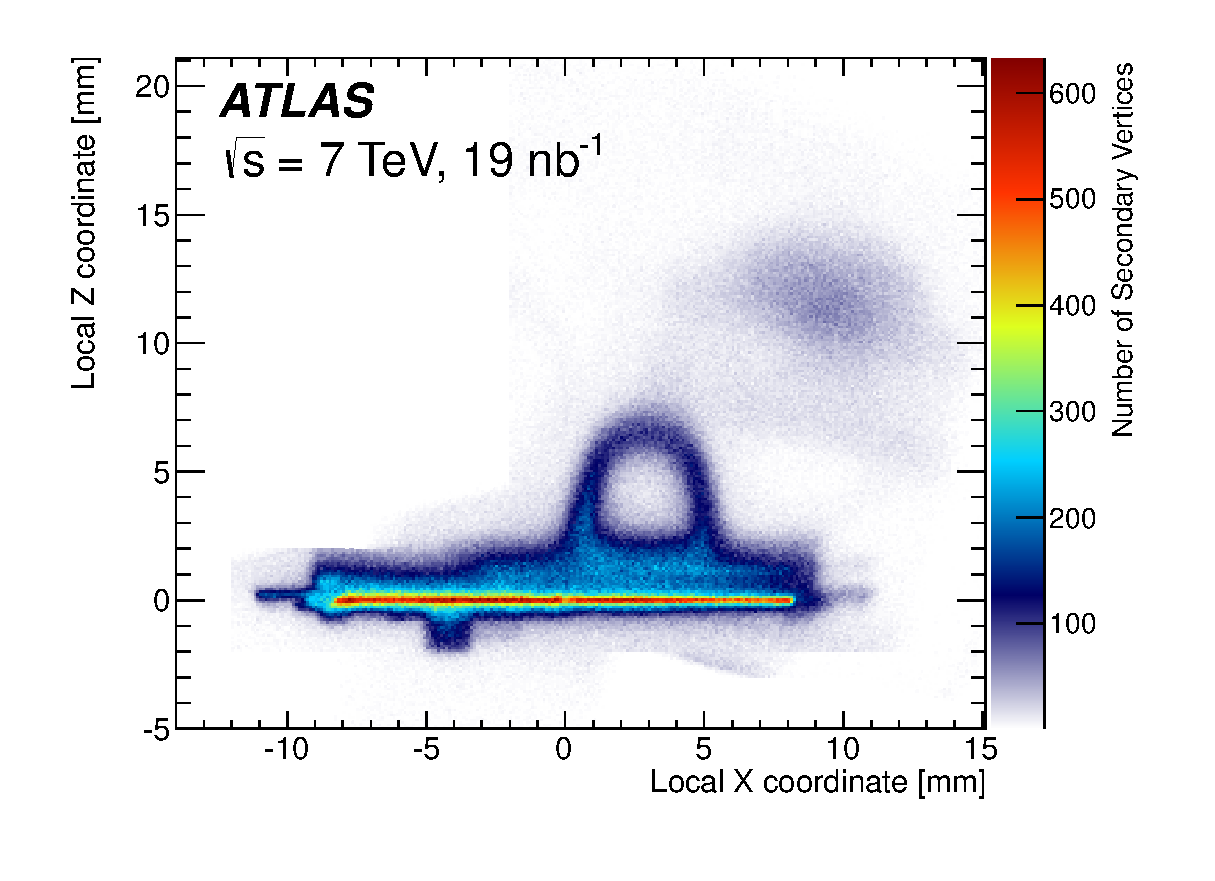
\includegraphics[width=.9\linewidth]{figures/theory/fig_10a.eps}
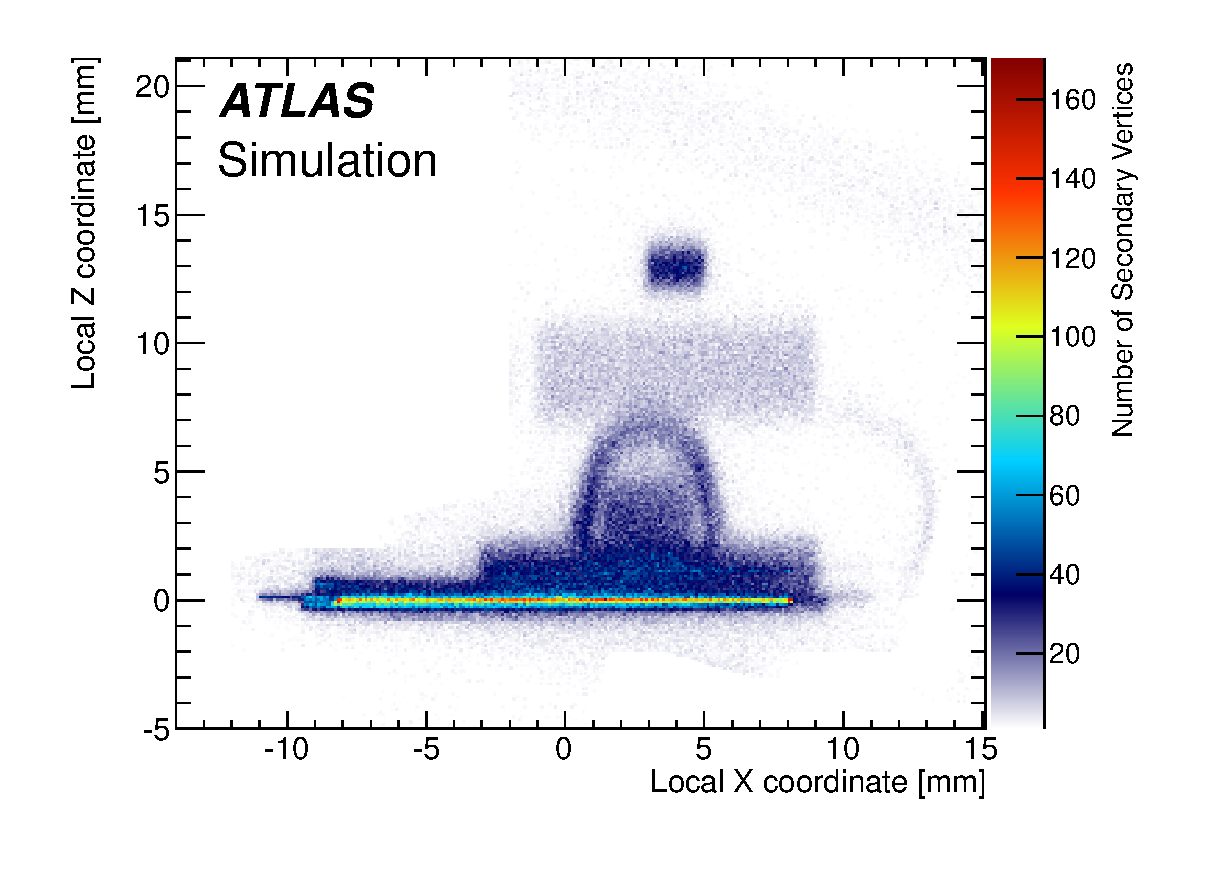
\includegraphics[width=.9\linewidth]{figures/theory/fig_10b.eps}
\caption{Number of secondary vertices in a module in the first layer of the pixel detector in data (top) and \ac{MC} (bottom). There are more events in the data than the \ac{MC} \cite{PERF-2015-06}.}
\label{fig:geant}
\end{figure}
\end{centering}

Custom \ac{ATLAS} code converts the energy deposited in active sensors into signals that resemble the expected detector response. These responses are typically very complicated with many parameters, and are frequently iterated on to best match the data. Electronic noise must also be added to correctly approximate the operating conditions of the detector. Additional alterations to this signal translation, including dead sensors and misalignments of the detector, can also be added at this stage. 

Once the simulated particles have been converted into detector signals, the same reconstruction software used on data can be used on the \ac{MC}, converting the detector signals back into particle interpretations. This reconstruction process is described in \autoref{ch:reconstruction}. The original information about the particles from the generator, referred to as \textit{truth} information, is also kept, and can be compared to the reconstruction output to study its efficacy.




